% !TEX root = ../Main.tex
Studying the Inertial electrostatic confinement fusor at DTU. Measurements of neutron counts and the spectral line width are made as a function of the voltage and current. To this, the emission spectrum of the gas are also measured.
\subsection{Plasma light emission and spectral line}
When doing spectroscopy on a plasma of an unknown gas. Optical dispersion splits up the spectrum of light into lines which are then recorded using a detector. This detector measures the frequency/wavelength of the light and the intensity of the light. Thus a plot with the wavelength along the x-axis vs the intensity along the y-axis are produced. For our recordings a typical spectrum looked like that of \cref{SPEC}.
\begin{figure}[H]
	\centering
	\resizebox{\textwidth}{!}{
		\begin{tikzpicture}
			\begin{axis}[
					width=\textwidth,
          height=\axisdefaultheight,
					title={Spectrum of light from fusion in the fusor},
					use units,
					x unit prefix=n, x unit=m,
					y unit=A.U.,
					xlabel=Wavelength,
					ylabel=Intensity,
					ymajorgrids=true,
					grid style=dashed,
					%scaled y ticks=manual:{\(10^{-9}\)}{\pgfmathparse{#1*10^9}}
				]
				\addplot[color=red] table {Data/SpectrumData.txt};
			\end{axis}
		\end{tikzpicture}
	}
	\caption{Spectrum of light from fusion in the fusor}
	\label{SPEC}
\end{figure}
Each peak correspond with a constituent gas in the fusor.
The peaks present on the spectrum are subject to broadening effects. Considering the Doppler effect, each photon's frequency will be shifted since the particles (which are the emitters) are moving at fast speeds (the Doppler shift increases with speed). Therefore if each particle where moving in the same direction the entire intensity peak would be shifted. But since the particles are moving more or less isotropic around the centre of the device, the peaks are not shifted but rather broadened around the normal emission wavelength. To this it is also noted that the Doppler broadening increases if particles are moving faster.\\
Considering \cref{fig:SPEC}, a spectrum is shown with central wavelengths around \SI{656}{\nano\meter}, \SI{486}{\nano\meter} and \SI{433}{\nano\meter} which correspond to accepted values of hydrogen light emission wavelengths\footnote{\href{https://en.wikipedia.org/wiki/Hydrogen_spectral_series}{``Hydrogen spectral series'' - Wikipedia (Visited January \nth{22})}}. Meanwhile the spectral lines of Deuterium only differs by a factor of $1.000272$\footnote{\href{https://en.wikipedia.org/wiki/Deuterium#Spectroscopy}{``Deuterium\#Spectroscopy'' - Wikipedia (Visited January \nth{22})}}, which will not be detected using our methods. There are other peaks but those peaks are due to noise from impurities etc.\\
Since the speed of the particles increases with the voltage we expect the line broadening to do the same since $\sigma=\lambda_{0}/c\, v_{\mathrm{1D}}$. While there seems to be enormous uncertainties on the hydrogen measurements, \cref{Vsigma} shows a tendency to increase for both hydrogen and deuterium. Disregarding outliers, the hydrogen also seems to have a wider spectral line than deuterium which makes sense due to the mass difference between the species. Meanwhile the uncertainties seen might be due to differences in pressure which leads to differences in kinetic energy lost per time. Other uncertainties are most likely also present.
\begin{figure}
    \centering
    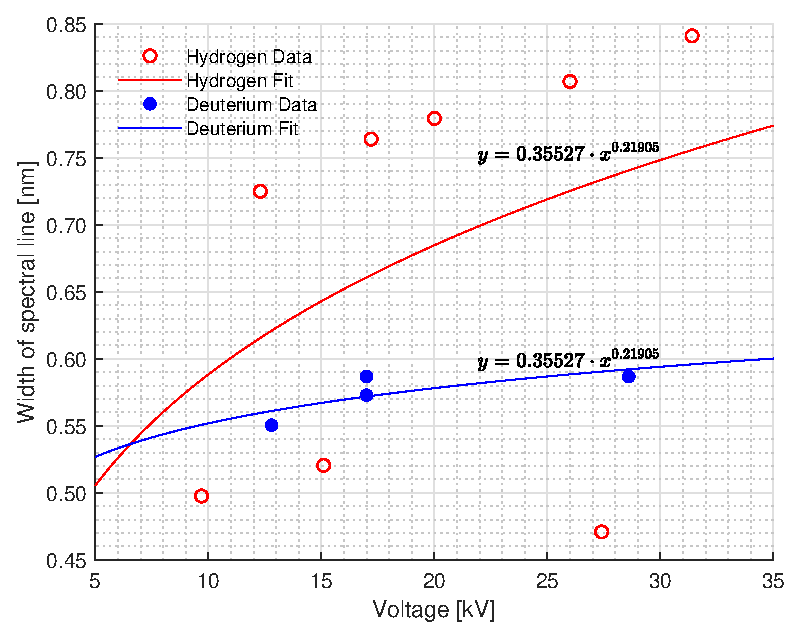
\includegraphics[width=.7\textwidth]{MatlabFigures/Asign3/VSigma.eps}
    \caption{The spectral line width as a function of applied voltage}
    \label{Vsigma}
\end{figure}
For the width of a spectral line, it is known that:
\begin{align}
    \sigma = \Delta\lambda = \frac{\lambda_0}{c} v_{\mathrm{1D}}\label{sigma1d}
\end{align}
So for the obtained widths the velocities can be estimated via \cref{sigma1d}. Once these points are obtained a curve is fitted to it. The fit is assumed to be linear as velocity is proportional to voltage applied. The kinetic energies are also estimated via:
\begin{align}
    KE = \frac{1}{2}mv^2\label{KE}
\end{align}
These points are also estimated and plotted along with a fit. The fit is assumed to be some constant times the square root of the voltage as as isolated from \cref{KE}. This is done for both hydrogen and deuterium. The plot can be seen in \cref{MF}.
\begin{figure}
    \centering
    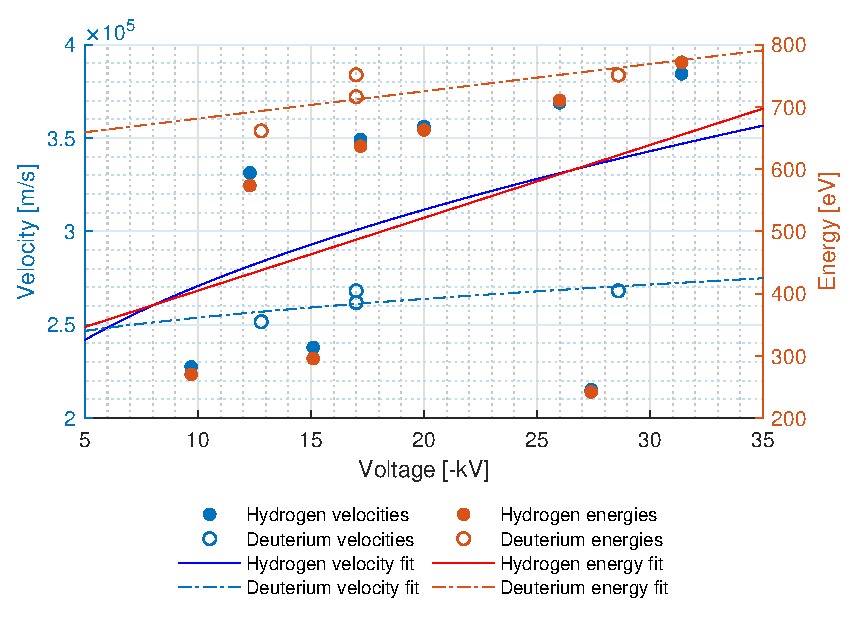
\includegraphics[width=.7\textwidth]{MatlabFigures/Asign3/KineticVelo.eps}
    \caption{The estimated velocities and kinetic energies for hydrogen and deuterium as functions of applied voltage}
    \label{MF}
\end{figure}
The four fits were computed to be:
\begin{align}
    \qq{Velocity for hydrogen:}& v = 3.12\times10^4 \sqrt{x}+1.72\times10^5 \\
    \qq{Velocity for deuterium:}& v = 0.7666\times10^4\sqrt{x}+2.295\times10^5\\
    \qq{Kinetic energy for hydrogen:}& KE = 11.7x+287.7\\
    \qq{Kinetic energy for deuterium:}& KE = 4.387x+637.3
\end{align}
with $x$ being the applied voltage. Of course the uncertainties from \cref{Vsigma} carries over which is unfortunate. We expected the deuterium and hydrogen energies to be equal which was not the case, but the velocity of hydrogen seems to be larger than the deuterium atoms which is to be expected.
\subsection{Neutron production rate}
The fusion reaction rate should increase with voltage and current where approximately every second reaction produce a neutron. Measurements of the neutron production rate are made and seen in \cref{neutron}. It is important to note that only 5 measurements are made, so the sample size will be very small. There are 3 parameters that varies throughout the measurements which makes it hard to say anything about the data. There is an unknown dependency on the pressure since an increasing pressure will decelerate the particles overall, but it will also increase the amount of fuel available. The pressure varies from $\SI{1.4}{\mu\Bar}$ to $\SI{2}{\mu\Bar}$. This should have an effect on the neutron rate, but let us disregard that fact for now. The data suggests that a current of $\SI{6}{\milli\ampere}$ is needed to get decent reaction rates when the voltage is in the ranges measured. On top of that, the data also suggests that the voltage needed is between $\SI{24}{\volts}$ and $\SI{28}{\volts}$. Note that the last suggestion is made at an approximately constant pressure.\\
Calculating the total neutron flux at the detector and the total neutron production rate is trivial given Cts./s,  $\eta_{\mathrm{eff.}}=15\‰$, $A_{\mathrm{det}}=\SI{6e-5}{\meter\squared}$ and $R_{\mathrm{det}}=\SI{0.5}{\meter}$.

\begin{align}
    \Gamma_{\mathrm{n}}=\frac{\mathrm{Cts.}}{\mathrm{s}}\,\frac{1}{\eta_{\mathrm{det}}}\,\frac{1}{A_{\mathrm{det}}} 
\end{align}
And $\mathrm{n}/\mathrm{s}=4\,\pi\, R_{\mathrm{det}}\,\Gamma_{\mathrm{n}}$. Now the power is equal to the product of the current and voltage but there is a voltage drop across the resistor bank which must be taken into account. Meanwhile the fusion power $P_{\mathrm{fusion}}=\mathrm{n}/\mathrm{s}\, (E_{\mathrm{n}}+E_{\alpha})$ with $E_{\mathrm{n}},\,E_{T}$ being the energy release of the reaction that results in a neutron and a tritium particle respectively(disregarding the other resulting particles).






\begin{table}[h!]
\begin{tabular}{llllllll}
\toprule
p($\si{\mu}$Bar) & I(mA) & V(-kV) & P(W) & Cts./s & $\Gamma_{\mathrm{n}}(\SI{}{\per\second\per\meter\squared})$ & n/s  & Q($\SI{e-6}{})$ \\ \midrule
2     & 12    & 17     & 194  & 0.689 & \SI{0.766e5}{} & \SI{2.41e5}{} & 1.45\\
1.7   & 9     & 24     & 210  & 0.891 & \SI{0.99e5}{} & \SI{3.11e5}{} & 1.73\\ 
1.6   & 7     & 28     & 193  & 2.106 & \SI{2.34e5}{} &  \SI{7.35e5}{} & 4.45\\ 
1.4   & 3     & 32     & 95.4   & 0.295 & \SI{0.328e5}{} & \SI{1.03e5}{} & 1.26\\ 
1.4n  & 6     & 33     & 195  & 1.725 & \SI{1.92e5}{} &  \SI{6.02e5}{} & 3.61\\
\bottomrule
\label{neutron}
\end{tabular}
\caption{Table containing the measured parameters for deuterium.}
\end{table}







